\documentclass{beamer}

% {{{ beamer stuffs
\setbeamertemplate{footline}[frame number]
\beamertemplatenavigationsymbolsempty%
\logo{
\includegraphics[height=4mm]{fig/LogoEnseeiht.png}}
\usetheme{Montpellier}
\usecolortheme{dolphin}
% }}}

\usepackage{fontspec}
\usepackage{hyperref}
\usepackage{pdflscape}

\usepackage{tikz}
\usetikzlibrary{shapes}

\title{CRAPS Kernel}
\subtitle{Final presentation}
\author{
       Maxime Arthaud
  \and Korantin Auguste
  \and Martin Carton
  \and Étienne Lebrun
}
\titlegraphic{
\includegraphics[width=0.5\textwidth]{fig/LogoEnseeiht.png}}
\date{March 13, 2015}

\begin{document}
  \begin{frame}[plain]
    \titlepage%
  \end{frame}

  \begin{frame}[plain]
    \tableofcontents
  \end{frame}

  \section{The project}
    \begin{frame}{Presentation}
      \begin{itemize}
        \item Implement a basic operating system on CRAPS:
          \begin{itemize}
            \item processor architecture developed by Jean-Christophe
              Buisson for first year students
            \item runs on a Nexys2 board
          \end{itemize}
        \item Goal: make a operating system course
          \begin{itemize}
            \item based on what student know
            \item adding a continuity in courses
            \item showing students how a basic operating system works
          \end{itemize}
      \end{itemize}
    \end{frame}

    \begin{frame}[plain]
      \begin{figure}
        \centering
        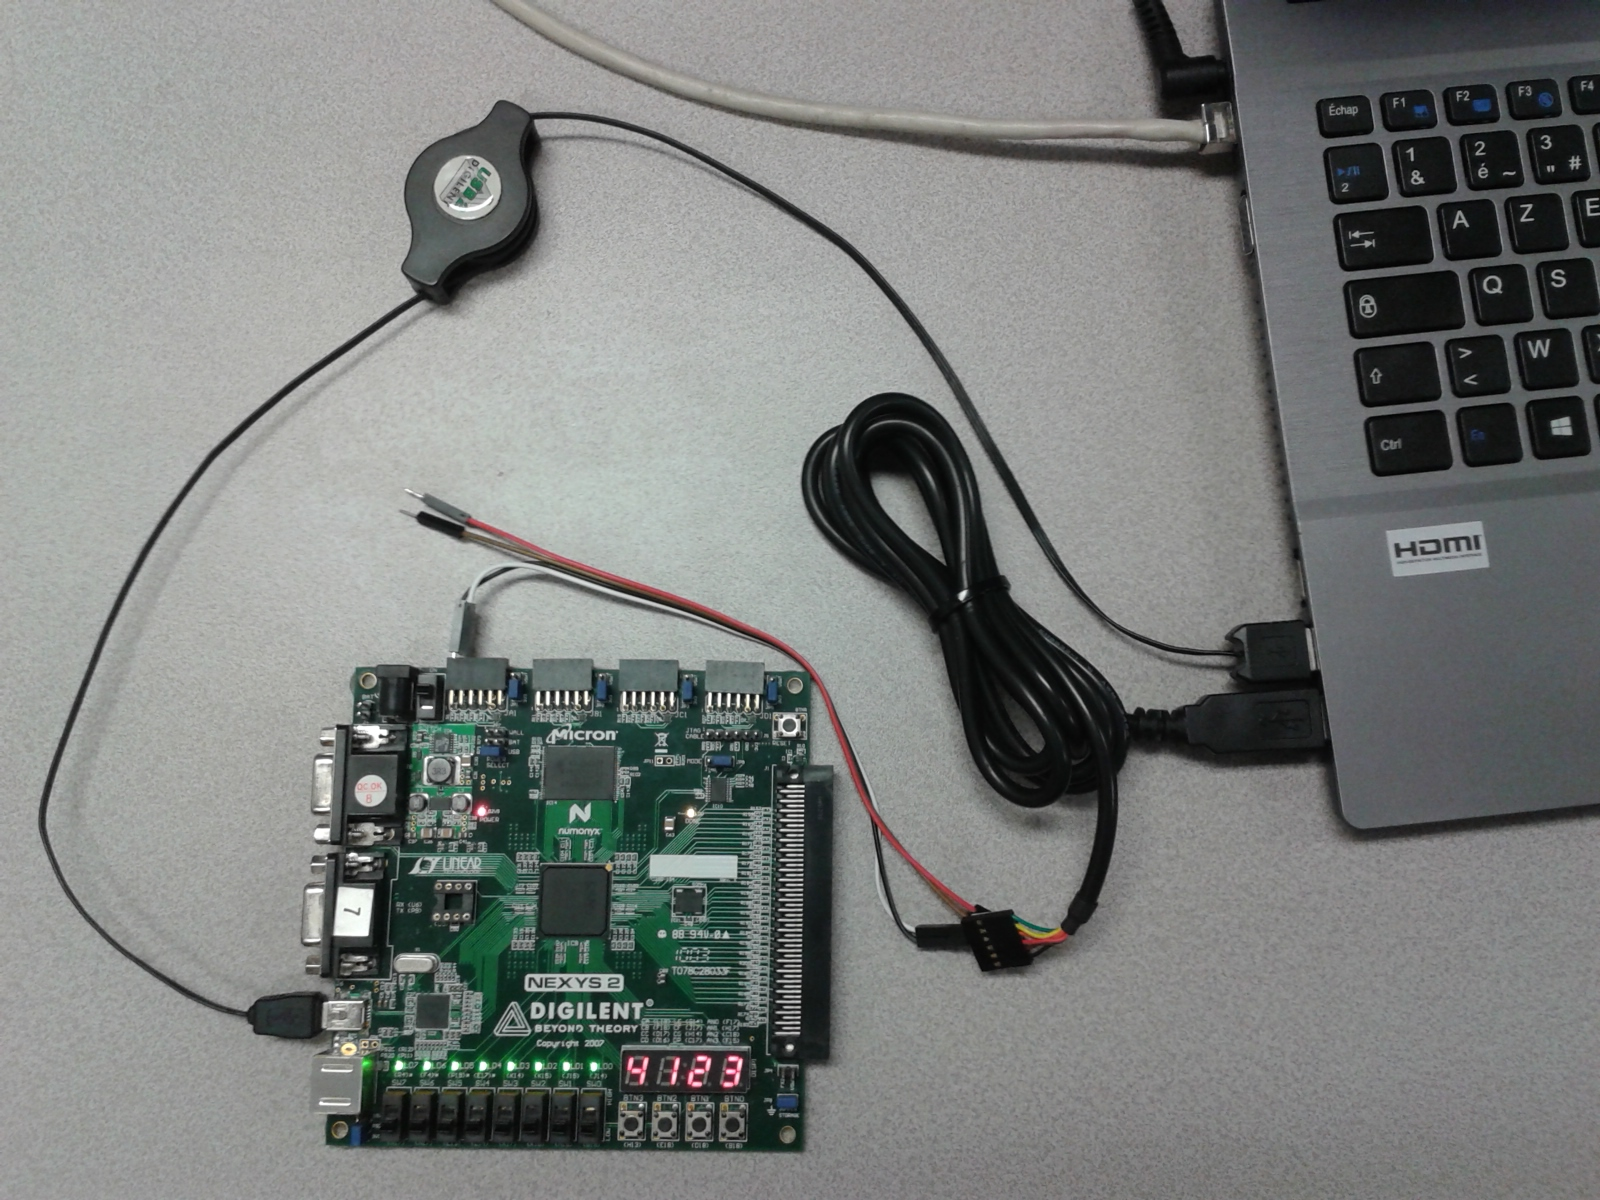
\includegraphics[width=\textwidth, keepaspectratio]{fig/Nexys2.jpg}
        \caption{A Nexys2 board}
      \end{figure}
    \end{frame}

  \section{Project Management}
    \subsection{Team}
      \begin{frame}{Team Organization}
        \begin{itemize}
          \item Korantin Auguste: responsible of development
          \item Maxime Arthaud: responsible of tests
          \item Martin Carton: \textit{project leader}
          \item Étienne Lebrun: \textit{quality manager}
        \end{itemize}
      \end{frame}

      \begin{frame}{Team Management}
        Quite free, working on what we like, when we like.

        \pause
        \begin{figure}
          \centering
          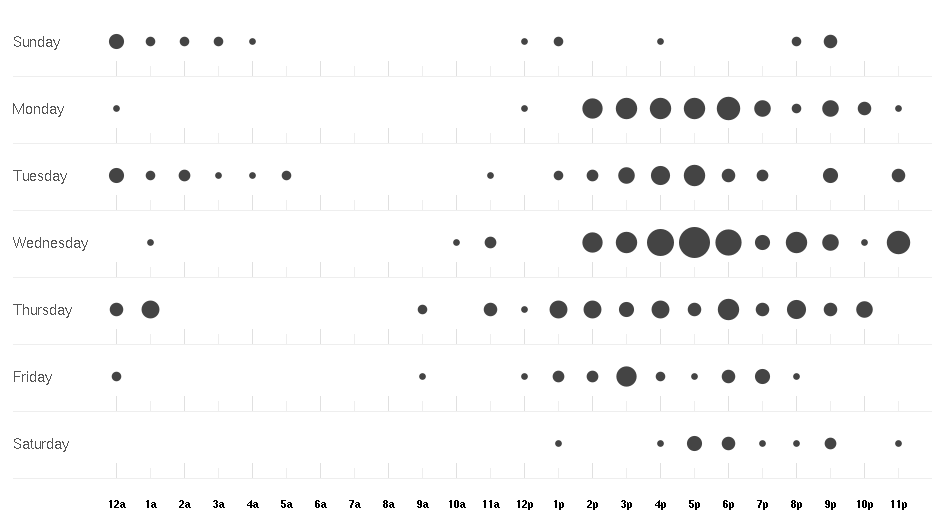
\includegraphics[width=0.9\textwidth]{fig/punchcard.png}
        \end{figure}
      \end{frame}

    \subsection{Project Organization}
      \begin{frame}{Risks Management}
        We have identified three risks and mitigated them:
        \begin{itemize}
          \item A FPGA might be damaged: we need more
          \item The OS might be too big to fit in the memory: we will need more
          \item The serial port might be too slow
        \end{itemize}
      \end{frame}

      \begin{frame}{Actions Management}
        We used a spreadsheet to manage the actions:
          \includegraphics[width=0.9\textwidth,keepaspectratio]
                          {Actions/ActionManagement.pdf}
      \end{frame}

      \begin{frame}{Specifications}
        \begin{itemize}
          \item First week of the project
          \item We identified three main tasks:
            \begin{itemize}
              \item The compiler
              \item The modifications to the processor
              \item The kernel
            \end{itemize}
          \end{itemize}
      \end{frame}

      \begin{frame}{Task Repartition and Planning}
          We used an incremental process, adding features one after another:
          \begin{enumerate}
            \item Write a simple scheduler
            \item Add communications using serial port
            \item Handle dynamic program loading
          \end{enumerate}

          We wrote a planning taking finish-to-start constraints into account.
      \end{frame}

      \begin{frame}[plain]
        \begin{figure}
          \includegraphics[height=\textheight, width=\textwidth, keepaspectratio]
                          {build/Gantt.pdf}
        \end{figure}
      \end{frame}

      \begin{frame}{Test Means}
        Not fully automated because of the constraints of the project:
        \begin{itemize}
          \item hardware: need to manually load test code and test it via the
            monitor
          \item compiler: some automated tests test the compiler itself, but the
            generated code has to be tested manually and it is impossible to be
            exhaustive
          \item kernel: need to use the monitor as well, outputs use 7-segment
            display, switches, etc.
        \end{itemize}

        Creation of a command line tool to load code more easily.
      \end{frame}

      \begin{frame}{Deliverables}
        \begin{itemize}
          \item Documentation and manual for students and teachers
            \begin{itemize}
              \item What we changed
              \item How to use our tools
              \item The syntax of our language
              \item \dots
            \end{itemize}
          \item Kernel, compiler, new processor
          \item Reports, abstracts
          \item Software Development Plan, Specifications, Test Plan
        \end{itemize}
      \end{frame}

  \section{Implementation}
    \begin{frame}
      \begin{figure}
        \centering
        \includegraphics[height=\textheight]{build/big_picture_fromsvg.pdf}
      \end{figure}
    \end{frame}

    \subsection{Kernel}
      \begin{frame}{Kernel introduction}
        Purpose of a kernel:
        \begin{itemize}
          \item memory management (dynamic allocation)
          \item scheduling and process management
          \item I/O (communication)
        \end{itemize}
      \end{frame}

      \begin{frame}{Shell}
          Need to interact with the OS.
          
          We want to:
          \begin{itemize}
            \item launch/stop programs
            \item know the state of the processes
          \end{itemize}
      \end{frame}

      \begin{frame}{Scheduler}
        Needed for time sharing, to run multiple process in ``parallel'' on the
        CPU.

        \begin{figure}
            \centering
            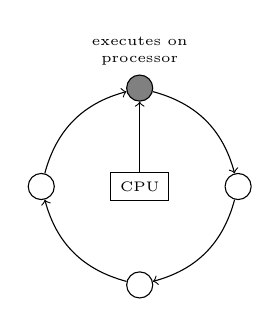
\begin{tikzpicture}[auto, ->, node distance=1.25cm]
            \node[auto] (CPU) [draw, style={font=\tiny}] {CPU};

            \node[auto] (A)   [draw, ellipse, above of=CPU, fill=gray,
            label={[align=center, style={font=\tiny}]executes on\\processor}] {};
            \node[auto] (B)   [draw, ellipse, right of=CPU] {};
            \node[auto] (C)   [draw, ellipse, below of=CPU] {};
            \node[auto] (D)   [draw, ellipse, left  of=CPU] {};

            \path (CPU) edge (A);

            \path (A) edge [bend left] (B);
            \path (B) edge [bend left] (C);
            \path (C) edge [bend left] (D);
            \path (D) edge [bend left] (A);
            \end{tikzpicture}
        \end{figure}

        Needed to make ``context switch'': change the current process.
      \end{frame}

      \begin{frame}{Memory Management}
        \begin{itemize}
          \item We need to be able to dynamically allocate memory
          \item In modern computers: virtual memory (segmentation and pagination)
            \begin{itemize}
              \item Too complicated
            \end{itemize}
          \item We just need three functions: \texttt{malloc}, \texttt{free},
            \texttt{realloc}
        \end{itemize}
      \end{frame}

      \begin{frame}[plain]
        \begin{figure}
          \begin{minipage}[c]{0.5\textwidth}
            \caption{Memory layout}
          \end{minipage}\hfill
          \begin{minipage}[c]{0.5\textwidth}
            \includegraphics[height=\textheight]{build/memory_layout_fromsvg.pdf}
          \end{minipage}
        \end{figure}
      \end{frame}

    \subsection{Processor Changes}

          \begin{frame}{Extending the Processor}
          Pre-existing version of CRAPS not totally adapted to our needs:
          \begin{itemize}
            \item Not enough memory
            \item No external communications
            \item No proper interrupts
          \end{itemize}
      \end{frame}

      \begin{landscape}
        \begin{frame}[plain]
            \includegraphics[scale=0.22]
                            {build/micromachine_old_fromsvg.pdf}

        \end{frame}
        \begin{frame}[plain]
            \includegraphics[scale=0.22]
                            {build/micromachine_updated_fromsvg.pdf}

        \end{frame}
      \end{landscape}

      \begin{frame}{Original Sequencer}
          \begin{figure}
            \centering
            \makebox[\textwidth][c]{
              \includegraphics[scale=0.3]
                                {build/sequencer_old_fromsvg.pdf}
            }
          \end{figure}
      \end{frame}

      \begin{frame}{After updates}
        \begin{figure}
          \centering
          \makebox[\textwidth][c]{
            \includegraphics[scale=0.21]
                           {build/sequencer_updated_fromsvg.pdf}
          }
        \end{figure}
      \end{frame}

      \begin{frame}{Adding Memory}
          Three possibilities:
          \begin{itemize}
            \item Extend the RAM module inside the FPGA
            \item Try to use the flash memory
            \item Access the external 16Mb RAM chip
        \end{itemize}

          Time consuming because of our lack of knowledge
      \end{frame}

      \begin{frame}{Block RAM}
        Extend the RAM module inside the FPGA
          \begin{itemize}
            \item Up to 63 kB available in dedicated Block RAM
            \item Requires Synchronised access
            \item Caused timing issues due to reading delay
                \begin{itemize}
                  \item Add a step in the sequencer to wait for the read value
                \end{itemize}
           \end{itemize}
      \end{frame}

      \begin{frame}{Flash Memory}
        Try to use the flash memory
        \begin{itemize}
          \item Caution!
          \item Quite complex communication protocol
        \end{itemize}
        \pause
        Finally, does not suit our needs because of inherent limitations
      \end{frame}

      \begin{frame}{External RAM}
        \begin{itemize}
          \item Easier to communicate with
          \item Word size discrepancy with our processor
        \end{itemize}
      \end{frame}

      \begin{frame}{Serial Port}
        To communicate with the computer we used a serial port.

        \pause
        We had to modify the processor:
        \begin{itemize}
          \item Add a new built-in module in SHDL
          \item Add a new interrupt in the processor
          \item Map the module to memory
        \end{itemize}

        \pause
        We had some problems:
        \begin{itemize}
          \item the module can cause the synthesis to fail (too complex?)
          \item the communication is slow, we can lose data
        \end{itemize}
      \end{frame}

      \begin{frame}{Interrupts}
        \begin{itemize}
          \item Add an interrupts module, that keeps the state of each interrupt
          \item Use a priority encoder
          \item The sequencer checks if there is an unhandled interrupt with a
            higher priority than the current execution level
          \item Interrupt table at position 1
        \end{itemize}
      \end{frame}

      \begin{frame}{Other Modifications}
        \begin{itemize}
          \item Add more registers:
            \begin{itemize}
                \item New special purpose register for PIC and new purpose for
                  the PSR
                \item Up to 19 general purpose registers can be used be the
                  compiler, all 32 registers are now mapped
            \end{itemize}
          \pause
          \item Add a test-and-set instruction
            \begin{itemize}
                \item Working but finally not used
            \end{itemize}
        \end{itemize}
      \end{frame}

    \subsection{Compiler}
      \begin{frame}{Why we need a compiler}
        % TODO martin: medium picture

        \begin{itemize}
          \item Very practical for the student to code.
          \item We can't write all the operating system in CRAPS assembly.
          \item But the generated code is less time/memory efficient.
        \end{itemize}

        We made a compiler, based on our second-year courses and the compiler
        generator of Mr.\ Gandriau, EGG.
      \end{frame}

      \begin{frame}{Dynamic Loading}
      \end{frame}

      \begin{frame}{Compiler}
        \begin{itemize}
          \item Various optimizations
          \item A more complete language
        \end{itemize}
      \end{frame}

  \section{Final Result}
    \begin{frame}{Various processes}
      \begin{itemize}
        \item The shell (most important)
        \item Counter
        \item LEDs
        \item \dots and dynamic loading!
      \end{itemize}
    \end{frame}

    \begin{frame}{Demo}
      \begin{itemize}
        \item The CRAPS processor is already on the board
        \pause
        \item Loading the kernel using the monitor
      \end{itemize}
      \begin{figure}
        \centering
        \makebox[\textwidth][c]{
          \includegraphics[width=10.5cm]{build/demo_load_fromsvg.pdf}
        }
      \end{figure}
      \pause
      \begin{itemize}
        \item Using the serial port with the shell task
        \pause
        \item Load a dynamic task
      \end{itemize}
    \end{frame}

  \section{Conclusion}
    \begin{frame}{Improvements}
    \end{frame}

    \begin{frame}{Conclusion}
    \end{frame}

  \section{Questions}
    \begin{frame}
      Any questions?
    \end{frame}
\end{document}
